% !TEX root = ../PRACA_MAIN.tex
\section{Metodyka Badań}

W niniejszym rozdziale przedstawiono kompleksowy protokół badawczy oraz szczegółowy aparat matematyczny wykorzystanych algorytmów rekomendacyjnych. Omówiono również specyfikę  środowiska wykonawczego, proces przygotowania i binarizacji zbioru danych oraz zastosowaną procedurę walidacji i ewaluacji jakości proponowanych propozycji rankingowych.

\subsection{Środowisko wykonawcze}

W celu standaryzacji protokołu ewaluacji wyników i przygotowania danych oraz dla zapewnienia maksymalnej powtarzalności wykorzystywanych algorytmów eksperymenty badawcze zdecydowano przeprowadzić z wykorzystaniem zunifikowanej biblioteki \foreignlanguage{english}{RecBole} (wersja 1.1.1) \footcite{zhaoRecBoleUnifiedComprehensive2020}. Biblioteka ta, oparta na frameworku \foreignlanguage{english}{PyTorch}, stanowi współcześnie standard badawczy w dziedzinie systemów rekomendacyjnych, łącząc w ramach jednolitej architektury modułowej cztery kluczowe komponenty: moduł konfiguracji, moduł danych, interfejsy modeli oraz zoptymalizowany moduł ewaluacji.

Sposób funkcjonowania ramki \foreignlanguage{english}{RecBole} opiera się na ściśle zdematerializowanej i zorientowanej na obliczenia GPU architekturze potokowej (ang. \foreignlanguage{english}{\textit{pipeline architecture}}). Przepływ danych i wykonanie eksperymentu wewnątrz biblioteki realizowane jest w następujących etapach:

\begin{enumerate}
    \item Moduł Konfiguracji (\foreignlanguage{english}{\textit{Configuration Module}}): Odpowiada za scalanie ustawień eksperymentalnych z hierarchicznie nakładanych źródeł: plików konfiguracyjnych \foreignlanguage{english}{YAML}, parametrów przekazywanych z wiersza poleceń oraz bezpośrednich słowników języka Python. Moduł ten kontroluje rozmiar batcha, stopę uczenia, użyty optymalizator (np. Adam, SGD) oraz szczegółowe parametry poszczególnych modeli.
    \item Moduł Danych i Struktura Interaction (\foreignlanguage{english}{\textit{Data Module}}): Surowe zbiory danych przekształcane są w uniwersalny format tzw. plików atomowych (ang. \foreignlanguage{english}{\textit{Atomic Files}}) z rozszerzeniem \texttt{.inter} (zawierających relacje użytkownik-obiekt) oraz opcjonalnie \texttt{.user}, \texttt{.item} czy \texttt{.kg} (dla metadanych i grafów wiedzy). Wewnątrz środowiska dane są reprezentowane przez wyspecjalizowany obiekt Interaction, będący opakowaniem na słownik tensorów \foreignlanguage{english}{PyTorch} (\texttt{torch.Tensor}). Zapewnia to bezpośrednie i bezkosztowe przenoszenie całych pakietów danych do pamięci VRAM karty graficznej (\texttt{.to(device)}), eliminując wąskie gardła transferu pamięci RAM-VRAM.
    \item Moduł Modelu (\foreignlanguage{english}{\textit{Model Module}}): Wszystkie zaimplementowane algorytmy dziedziczą po zunifikowanych klasach bazowych (np. GeneralRecommender dla modeli filtracji kolaboracyjnej oraz KnowledgeRecommender dla modeli z grafami wiedzy). Wymaga to od każdego algorytmu zdefiniowania dwóch zunifikowanych interfejsów:
          \begin{itemize}
              \item calculate\_loss(interaction) -- wyliczanie wartości funkcji straty (np. \foreignlanguage{english}{BPR Loss} lub \foreignlanguage{english}{Binary Cross-Entropy}) w fazie propagacji wprzód podczas uczenia,
              \item predict(interaction) / full\_sort\_predict(interaction) -- wyznaczanie punktacji relewancji (\foreignlanguage{english}{\textit{scores}}) dla par użytkownik-obiekt w fazie predykcji.
          \end{itemize}
    \item Moduł Wykonania i Akceleracji Ewaluacji (\foreignlanguage{english}{\textit{Execution \& Evaluation Module}}): Pętla uczenia zarządzana jest przez obiekt Trainer, odpowiadający za automatyczny zapis punktów kontrolnych (\foreignlanguage{english}{\textit{checkpoints}}), wczesne zatrzymanie (\foreignlanguage{english}{\textit{early stopping}}) oraz optymalizację hiperparametrów.
\end{enumerate}

Środowisko uruchomieniowe przygotowano na podstawie systemu operacyjnego Windows 11 oraz interpretera języka Python (wersja 3.12) działającego w odizolowanym środowisku wirtualnym. Wszystkie parametry modeli oraz ustawienia eksperymentalne zostały natomiast zdefiniowane w postaci deklaratywnych plików konfiguracji \foreignlanguage{english}{YAML}. Rozwiązanie to gwarantuje pełną separację logiki eksperymentalnej od kodu źródłowego, ułatwiając rekonfigurowalność hiperparametrów, kontrolę wersji eksperymentów oraz bezproblemową powtarzalność uzyskanych wyników. Zastosowanie jednolitej ramki \foreignlanguage{english}{RecBole} eliminuje ponadto tzw. błędy niespójności implementacyjnej (ang. \foreignlanguage{english}{\textit{reproducibility crisis}}), gwarantując, że obserwowane różnice w wynikach wynikają wyłącznie z właściwości samych algorytmów.

\subsection{Opis i przygotowanie danych}

W części empirycznej niniejszej pracy do ewaluacji modeli rekomendacyjnych wykorzystano zbiór danych \foreignlanguage{english}{MovieLens 1M}, udostępniany przez grupę badawczą \foreignlanguage{english}{GroupLens Research} z \foreignlanguage{english}{University of Minnesota}. Wybór tego zbioru jest podyktowany jego powszechnym uznaniem w literaturze naukowej jako kanonicznego benchmarku w dziedzinie systemów rekomendacyjnych \footcite{harperMovieLensDatasetsHistory2016, heNeuralCollaborativeFilteringKwiecien032017, zhaoRecBoleUnifiedComprehensive2020}.

Przestrzeń badawczą definiuje trójka uporządkowana obejmująca:
\begin{itemize}
    \item zbiór wszystkich zarejestrowanych użytkowników, oznaczany symbolem $\mathcal{U}$ (gdzie $M = |\mathcal{U}|$ stanowi łączną liczbę użytkowników),
    \item zbiór wszystkich dostępnych w katalogu obiektów (filmów), oznaczany symbolem $\mathcal{I}$ (gdzie $N = |\mathcal{I}|$ stanowi łączną liczbę obiektów),
    \item zbiór zaobserwowanych historycznych interakcji, oznaczany symbolem $\mathcal{E}$ ($\mathcal{E} \subseteq \mathcal{U} \times \mathcal{I}$), reprezentujący zaobserwowane zdarzenia o liczebności $|\mathcal{E}|$.
\end{itemize}

W analizowanym zbiorze dane te przyjmują wartości: $M = 6\,040$, $N = 3\,706$ oraz $|\mathcal{E}| = 1\,000\,209$. Dokładne ustalenie wymiarów $M$ i $N$ jest kluczowe z punktu widzenia uczenia maszynowego, gdyż determinują one bezpośrednio rozmiary wejściowych słowników dla warstw osadzeń (\foreignlanguage{english}{\textit{embedding layers}}) w architekturach neuronowych i grafowych \footcite[sekcje 2.1, 3.2 oraz 3.4]{zhangDeepLearningBased2020}. W klasycznym ujęciu rzadkie wektory identyfikatorów użytkowników $\mathbf{v}_u \in \{0, 1\}^M$ (typu \foreignlanguage{english}{\textit{one-hot}}) oraz obiektów $\mathbf{v}_i \in \{0, 1\}^N$ są mapowane na gęste reprezentacje wektorowe $\mathbf{e}_u \in \mathbb{R}^k$ i $\mathbf{e}_i \in \mathbb{R}^k$ (gdzie $k \ll \min(M, N)$) poprzez mnożenie przez macierze wag osadzeń odpowiednio $\mathbf{P} \in \mathbb{R}^{M \times k}$ oraz $\mathbf{Q} \in \mathbb{R}^{N \times k}$.

Tradycyjny model danych rekomendacyjnych reprezentuje się jako dwuwymiarową macierz interakcji $\mathbf{R} \in \mathbb{R}^{M \times N}$, w której wiersze odpowiadają poszczególnym użytkownikom ($u \in \mathcal{U}$), a kolumny poszczególnym obiektom ($i \in \mathcal{I}$) \footcite[2]{suSurveyCollaborativeFiltering2009}. Stopień braku wypełnienia tej struktury opisuje wskaźnik rzadkości (\foreignlanguage{english}{\textit{sparsity rate}}), oznaczany symbolem $S \in [0, 1]$. Definiuje się go jako dopełnienie stosunku liczby faktycznie zaobserwowanych interakcji do teoretycznej maksymalnej liczby wszystkich możliwych powiązań w macierzy:
\begin{equation}
    S = 1 - \frac{|\mathcal{E}|}{M \times N}
\end{equation}

Dla wybranego zbioru danych stopień rzadkości wynosi $S = 95{,}53\%$, co oznacza, że jedynie $4{,}47\%$ komórek macierzy zawiera zaobserwowane wpisy. W środowisku VOD skrajna rzadkość jest zjawiskiem naturalnym --- pojedynczy widz jest w stanie zapoznać się jedynie z ułamkiem procenta całkowitej oferty platformy \footcite[19, 23]{checinskiSystemyRekomendacjiRemedium2023}. Skrajnie wysoki wskaźnik rzadkości stanowi podstawowe uzasadnienie metodologiczne dla odrzucenia prostych algorytmów pamięciowych ($k$-NN), które zmagają się z problemem braku wspólnych sąsiadów, na rzecz metod czynników ukrytych (SVD) \footcite[2, 3]{suSurveyCollaborativeFiltering2009, korenMatrixFactorizationTechniques2009} oraz propagacji osadzeń w sieciach grafowych \footcite[sekcja 3.4]{zhangDeepLearningBased2020}.

Interakcje na platformach streamingowych podlegają silnej asymetrii popytu opisanej rozkładem potęgowym (\foreignlanguage{english}{\textit{Power Law}}) \footcite[14--15, 105]{celmaMusicRecommendationDiscovery2010}. Charakterystyczną cechą tej asymetrii w systemach dystrybucji cyfrowej jest fakt, że skrajnie nieliczna, uprzywilejowana grupa najpopularniejszych pozycji skupia wokół siebie zdecydowaną większość całej aktywności w systemie, podczas gdy olbrzymia większość pozostałych obiektów odnotowuje znikome zainteresowanie ze strony odbiorców \footcite[93]{celmaMusicRecommendationDiscovery2010}. Badana przestrzeń danych jednoznacznie wykazuje zjawisko tzw. długiego ogona (\foreignlanguage{english}{\textit{Long-Tail Distribution}}), zaprezentowane na Rysunku \ref{fig:long_tail}.

\begin{figure}[h!]
    \centering
    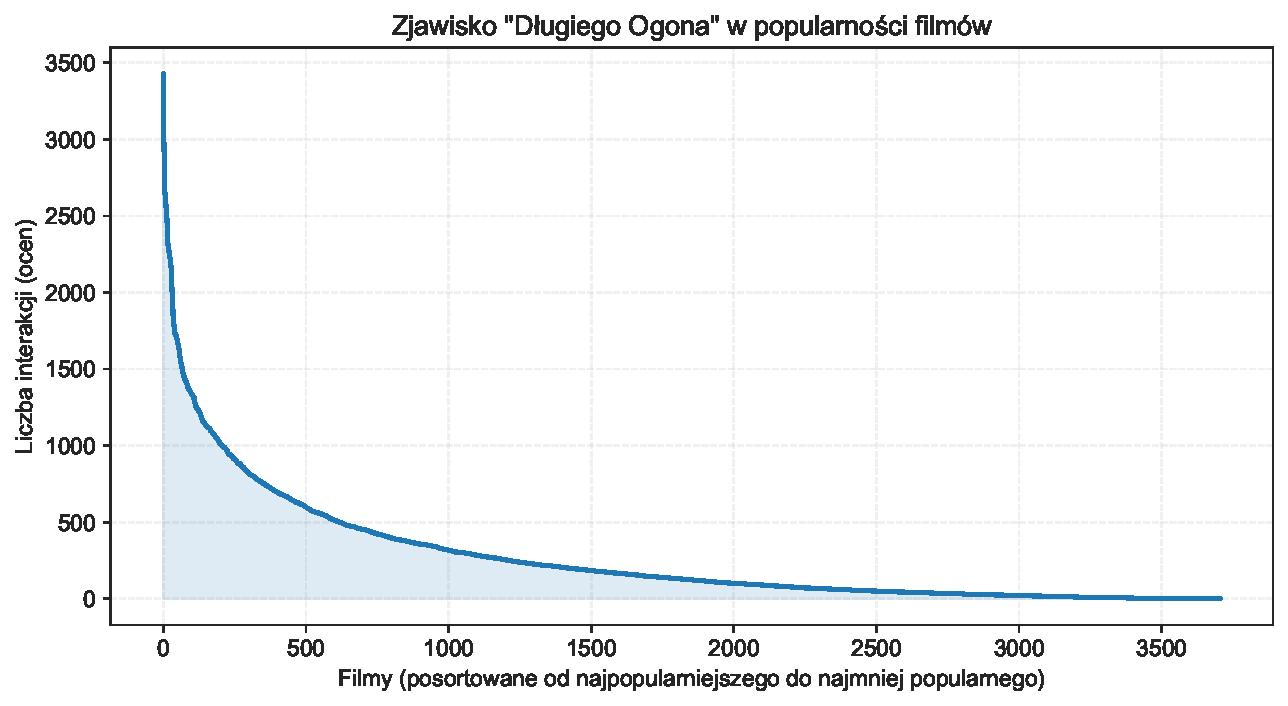
\includegraphics[width=0.85\textwidth]{img/movielens_long_tail.pdf}
    \caption{Rozkład popularności filmów w zbiorze MovieLens 1M przedstawiający zjawisko długiego ogona (\foreignlanguage{english}{\textit{Long-Tail Distribution}}).}
    \label{fig:long_tail}
    \vspace{1.5mm}

    {\raggedright \small \textbf{Źródło:} opracowanie własne.\par}
\end{figure}

Katalog filmowy dzieli się na dwie wyraźne strefy \footcite[100]{celmaMusicRecommendationDiscovery2010}:
\begin{itemize}
    \item \textbf{Głowę popytu (\foreignlanguage{english}{\textit{Head}}):} wąską grupę najpopularniejszych produkcji kinowych (tzw. hitów), które skupiają przeważającą część całkowitej liczby ocen w systemie. Tradycyjnie to ta część oferty była faworyzowana w erze analogowej ze względu na ograniczenia fizycznej przestrzeni sklepowej i wysokie koszty dystrybucji, które wymuszały na dystrybutorach selekcję wyłącznie pozycji o masowej popularności \footcite[14--15, 100]{celmaMusicRecommendationDiscovery2010}.
    \item \textbf{Długi ogon (\foreignlanguage{english}{\textit{Tail}}):} obszerną listę niszowych, mniej znanych lub starszych tytułów o niskiej częstotliwości odtworzeń. W dobie cyfrowej, po wyeliminowaniu fizycznych ograniczeń magazynowych i półkowych, cała ta niszowa oferta może pozostawać stale dostępna dla użytkowników, tworząc ogromną sumę małych rynków o bardzo wysokim potencjale zaspokajania specyficznych i zróżnicowanych gustów \footcite[100]{celmaMusicRecommendationDiscovery2010}.
\end{itemize}

Z biznesowego i funkcjonalnego punktu widzenia spersonalizowany system rekomendacyjny na rynku VOD musi potrafić trafnie proponować pozycje z długiego ogona, zapobiegając zjawisku monopolizacji uwagi widza wyłącznie przez najpopularniejsze hity \footcite[23]{checinskiSystemyRekomendacjiRemedium2023}. W dobie tzw. cyfrowej klęski urodzaju, gdy platformy streamingowe oferują tysiące filmów i seriali, użytkownicy stają w obliczu przeładowania informacyjnego, w którym samodzielne dotarcie do interesujących pozycji staje się wysoce utrudnione, a zapoznanie się z pełną ofertą katalogową jest fizycznie niemożliwe \footcite[19]{checinskiSystemyRekomendacjiRemedium2023}. Brak skutecznego mechanizmu personalizacji sprawia, że uwaga użytkowników koncentruje się wyłącznie na tytułach najgłośniejszych i powszechnie promowanych, co prowadzi do marnowania potencjału niszowej części biblioteki serwisu \footcite[19]{checinskiSystemyRekomendacjiRemedium2023}. Wdrożenie algorytmów zdolnych do eksploracji długiego ogona i kierowania uwagi widzów z obszaru głowy popytu ku pozycjom niszowym pozwala na pełniejsze wykorzystanie zasobów, zwiększa satysfakcję i lojalność odbiorców oraz maksymalizuje zaangażowanie w korzystanie z platformy \footcite[14--15, 23]{celmaMusicRecommendationDiscovery2010, checinskiSystemyRekomendacjiRemedium2023}.

Oryginalny zbiór MovieLens zawiera oceny jawne (\foreignlanguage{english}{\textit{explicit feedback}}) wyrażone w 5-stopniowej skali dyskretnej (od 1 do 5 gwiazdek). Choć oceny te dostarczają bardzo precyzyjnej i jednoznacznej informacji o stopniu satysfakcji użytkownika, w rzeczywistych systemach rekomendacyjnych współczesnych platform wideo występują one niezwykle rzadko. Wynika to z faktu, że czynność ta nakłada na odbiorcę dodatkowe obciążenie poznawcze i wymaga intencjonalnego działania po seansie, co zakłóca naturalną, bezwysiłkową konsumpcję treści --- większość widzów chce po prostu oglądać kolejne materiały, a nie dokonywać ich ewaluacji \footcite[452]{rendleBPRBayesianPersonalized2009}.

W konsekwencji głównym źródłem informacji dla algorytmów stają się ślady cyfrowe i interakcje dorozumiane (\foreignlanguage{english}{\textit{implicit feedback}}), takie jak odtworzenie filmu, czas jego oglądania, kliknięcie w miniaturę czy historia wyszukiwania \footcite[2]{suSurveyCollaborativeFiltering2009, checinskiSystemyRekomendacjiRemedium2023}. Dane te są gromadzone przez platformy całkowicie pasywnie, bez wysiłku ze strony widza, co pozwala na budowę znacznie większych i bardziej aktualnych zbiorów uczących, choć są one trudniejsze w interpretacji z uwagi na brak bezpośredniej deklaracji zadowolenia \footcite[452--453]{rendleBPRBayesianPersonalized2009}. Rozkład ocen jawnych w analizowanym zbiorze zaprezentowano na Rysunku \ref{fig:ratings_distribution}.

\begin{figure}[H]
    \centering
    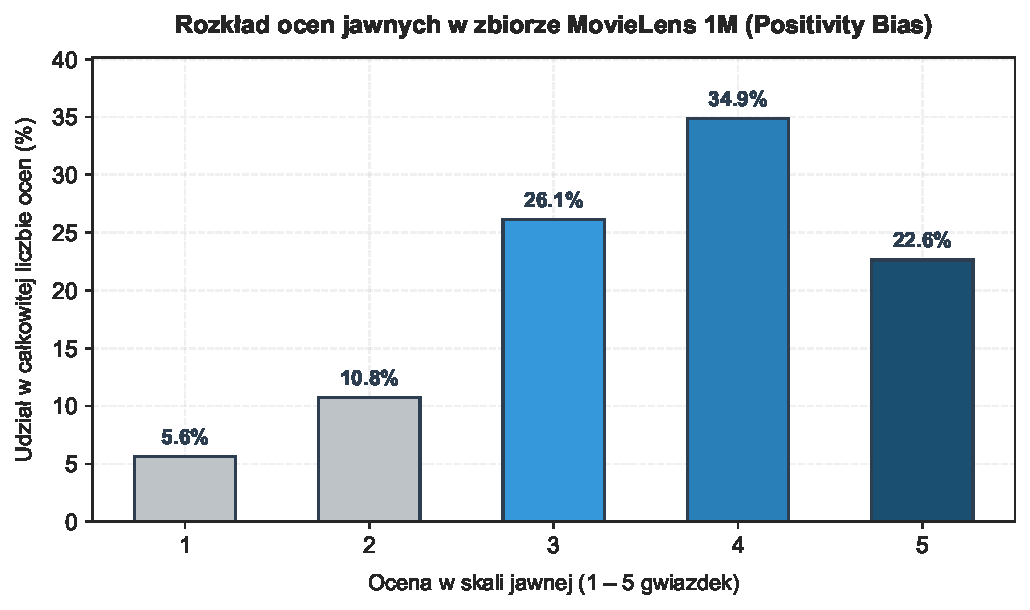
\includegraphics[width=0.82\linewidth]{img/movielens_ratings_distribution.pdf}
    \caption{Rozkład ocen jawnych w zbiorze MovieLens 1M obrazujący efekt zjawiska \foreignlanguage{english}{\textit{positivity bias}}}
    \label{fig:ratings_distribution}
    {\raggedright \small \textbf{Źródło:} opracowanie własne na podstawie danych z zestawu MovieLens 1M.\par}
\end{figure}

Analiza histogramu wykazuje silne skrzywienie pozytywne (\foreignlanguage{english}{\textit{positivity bias}}) -- użytkownicy znacznie chętniej oceniają filmy, które im się podobały, podczas gdy produkcje ocenione negatywnie są w logach niemal nieobecne (oceny 3, 4 i 5 stanowią ponad $80\%$ wszystkich wpisów). Zjawisko to jest bezpośrednią konsekwencją błędu selekcji; widzowie intuicyjnie wybierają do obejrzenia te tytuły, wobec których żywią już uprzednie pozytywne oczekiwania (np. ze względu na ulubiony gatunek czy obsadę), co wtórnie drastycznie ogranicza szansę na wystawienie niskiej noty \footcite[28]{celmaMusicRecommendationDiscovery2010}. W rezultacie obserwowany zbiór ocen jawnych nie odzwierciedla reprezentatywnego profilu gustu użytkownika wobec całego katalogu, a jedynie wobec jego wyselekcjonowanego ułamka \footcite[28]{celmaMusicRecommendationDiscovery2010}.

Zgodnie z metodologią zaproponowaną przez He i in. \footcite[7]{heNeuralCollaborativeFilteringKwiecien032017}, w celu dostosowania danych do realiów platform streamingowych dokonuje się przekształcenia binarnego oryginalnej macierzy ocen w macierz interakcji dorozumianych, oznaczaną jako $\mathbf{Y} \in \mathbb{R}^{M \times N}$ (gdzie $M = |\mathcal{U}|$ oznacza liczbę użytkowników, a $N = |\mathcal{I}|$ liczbę filmów). Zabieg ten pozwala na przekształcenie subiektywnego problemu regresji ocen w zadanie klasyfikacji binarnej (rekomendacji góry listy), co znacznie lepiej oddaje rzeczywiste zachowanie i procesy decyzyjne użytkowników w serwisach OTT, gdzie kluczowym wyborem jest decyzja o kliknięciu i rozpoczęciu odtwarzania danego tytułu \footcite[7]{heNeuralCollaborativeFilteringKwiecien032017}.

Przed przedstawieniem reguły dyskryminacyjnej zdefiniujmy elementy składowe wzoru:
\begin{itemize}
    \item $y_{ui}$ --- wartość wskaźnikowa określająca obecność zaobserwowanej relacji pomiędzy użytkownikiem $u \in \mathcal{U}$ a obiektem $i \in \mathcal{I}$,
    \item $y_{ui} = 1$ --- stan dodatni, oznaczający zarejestrowanie interakcji (np. wystawienie jakiejkolwiek oceny lub obejrzenie filmu),
    \item $y_{ui} = 0$ --- stan nieobserwowany, oznaczający brak zarejestrowanej akcji w logach systemowych.
\end{itemize}

Sformułowanie matematyczne funkcji binarnej przyjmuje postać:
\begin{equation}
    y_{ui} = \begin{cases} 1, & \text{jeśli zaobserwowano interakcję (użytkownik } u \text{ ocenił/obejrzał film } i\text{)} \\ 0, & \text{w przeciwnym razie (brak obserwacji)} \end{cases}
\end{equation}

Warto podkreślić, że wartość $y_{ui} = 0$ ma charakter wysoce niejednoznaczny semantycznie. Nie oznacza ona bowiem jawnej niechęci użytkownika do danego tytułu, lecz jedynie brak wiedzy o wchodzeniu w interakcję \footcite[2]{heNeuralCollaborativeFilteringKwiecien032017}. Użytkownik mógł nie obejrzeć filmu z powodów zupełnie niezależnych od jego gustu: mógł go nie zauważyć w katalogu, nie zostać na niego wyeksponowany przez interfejs platformy, bądź po prostu jeszcze na niego nie trafić \footcite[2]{heNeuralCollaborativeFilteringKwiecien032017, rendleBPRBayesianPersonalized2009}. Struktura ta stanowi fundamentalne wyzwanie w uczeniu maszynowym, gdyż zbiór danych nieobserwowanych ($y_{ui} = 0$) de facto reprezentuje jednocześnie rzeczywiste negatywne preferencje (użytkownik zna film, ale nie chce go obejrzeć), jak i potencjalne przyszłe interakcje dodatnie (użytkownik chętnie obejrzałby film, gdyby tylko dowiedział się o jego istnieniu), które model powinien poprawnie zidentyfikować i wybić na górę listy rekomendacji \footcite[453]{rendleBPRBayesianPersonalized2009}.


Rozkład aktywności użytkowników wykazuje duże zróżnicowanie -- od profilów okazjonalnych po użytkowników o skrajnie wysokiej liczbie obejrzanych pozycji. Aby wyeliminować zaburzenia wynikające ze skrajnie rzadkich profilów oraz pozycji znikających z katalogu bez historii ocen, zastosowano procedurę filtrowania typu $k$-\foreignlanguage{english}{\textit{core}} ($k = 5$) \footcite[7, sekcja 4.1.1]{heNeuralCollaborativeFilteringKwiecien032017}. Odrzucono wszystkich użytkowników oraz filmy posiadające mniej niż 5 zarejestrowanych interakcji. Operacja ta zapobiega występowaniu niemożliwych do wyuczenia trywialnych wektorów zerowych w warstwach embeddingów oraz stabilizuje proces wyznaczania normalizacji macierzy sąsiedztwa grafu dwudzielnego w modelach GNN \footcite[6, sekcja 2.1.1]{zhaoRecBoleUnifiedComprehensive2020}.

W celu zapewnienia ścisłej reprodukowalności eksperymentów i eliminacji błędów implementacyjnych, oczyszczone zbiory danych przekonwertowano do formatu Plików Atomowych (ang. \foreignlanguage{english}{\textit{Atomic Files}}) z rozszerzeniem \texttt{.inter}, stanowiącego standard wejściowy biblioteki RecBole \footcite[6, sekcja 2.1.2]{zhaoRecBoleUnifiedComprehensive2020}. Plik \texttt{.inter} przechowuje relacje w strukturze tabularycznej ze zdefiniowanymi typami pól \footcite[6, Tabela 3]{zhaoRecBoleUnifiedComprehensive2020}:
\begin{itemize}
    \item \texttt{user\_id:token} -- unikalny identyfikator użytkownika (sekwencja dyskretna),
    \item \texttt{item\_id:token} -- unikalny identyfikator filmu (sekwencja dyskretna),
    \item \texttt{rating:float} -- oryginalna ocena użytkownika (wykorzystywana pomocniczo),
    \item \texttt{timestamp:float} -- znacznik czasu interakcji.
\end{itemize}


Ewaluację modeli przeprowadzono w oparciu o proporcjonalny losowy podział danych (\foreignlanguage{english}{\textit{Ratio Splitting}}) w stosunku $80\% : 10\% : 10\%$ (odpowiednio: zbiór treningowy, walidacyjny i testowy), co stanowi standardowy protokół podziału danych typu \foreignlanguage{english}{\textit{ratio-based splitting}} obsługiwany przez bibliotekę RecBole \footcite[6, sekcja 2.1.1 oraz s. 7, sekcja 2.3.4]{zhaoRecBoleUnifiedComprehensive2020}.

Do trenowania modeli punktowych i parowych (Log Loss w NCF oraz BPR Loss w SVD/LightGCN) zastosowano procedurę próbkowania negatywnego (\foreignlanguage{english}{\textit{negative sampling}}). Dla każdej dodatniej pary $(u, i) \in \mathcal{E}$ losowano jednostajnie ze zbioru pozycji nieobserwowanych zestaw próbek negatywnych $(u, j) \in \mathcal{E}^-$ (gdzie $y_{uj} = 0$), przy zachowaniu stosunku $1:4$ (4 próbki negatywne na 1 pozycję dodatnią), co stanowi optymalny kompromis między stabilnością gradientu a czasem obliczeń \footcite[7, sekcja 4.1.2]{heNeuralCollaborativeFilteringKwiecien032017}. Zastosowanie elastycznej liczby próbek negatywnych (w optymalnym przedziale od 3 do 6) pozwala modelom optymalizowanym punktową stratą logarytmicznej na znaczące przełamanie ograniczeń klasycznych strat parowych typu BPR, które z natury parują wyłącznie jedną próbkę negatywną z dodatnią \footcite[8, sekcja 4.3]{heNeuralCollaborativeFilteringKwiecien032017}.



\newpage
Tabela \ref{tab:movielens_stats} przedstawia zbiorcze zestawienie parametrów statystycznych przygotowanego zbioru danych MovieLens 1M po przeprowadzeniu potoku przetwarzania.

\begin{table}[H]
    \centering
    \small
    \setlength{\tabcolsep}{6pt}
    \caption{Podsumowanie statystyczne zbioru danych MovieLens 1M wykorzystanego w eksperymentach}
    \label{tab:movielens_stats}
    \begin{tabular}{|l|c|}
        \hline
        \textbf{Parametr statystyczny}             & \textbf{Wartość dla zbioru MovieLens 1M (\texttt{ml-1m})} \\ \hline
        Liczba użytkowników ($|\mathcal{U}|$)      & 6\,040                                                    \\ \hline
        Liczba filmów ($|\mathcal{I}|$)            & 3\,706                                                    \\ \hline
        Liczba interakcji ($|\mathcal{E}|$)        & 1\,000\,209                                                \\ \hline
        Średnia liczba ocen na użytkownika         & 165{,}60                                                  \\ \hline
        Gęstość macierzy (\textit{Density})         & 4{,}47\%                                                  \\ \hline
        Rzadkość macierzy (\textit{Sparsity})       & 95{,}53\%                                                 \\ \hline
        Typ informacji zwrotnej                    & Interakcje dorozumiane (\textit{Implicit Feedback})       \\ \hline
    \end{tabular}
    \vspace{1.5mm}

    {\raggedright \small \textbf{Źródło:} opracowanie własne na podstawie danych MovieLens 1M.\par}
\end{table}

\subsection{Algorytmy filtrowania kolaboracyjnego}
\subsection{Algorytmy uczenia głębokiego}
\subsection{Algorytmy grafowych sieci neuronowych}
\subsection{Metryki oceny}